\section{Apendice}

\subsection{Requerimientos del software}
Para poder utilizar el parser es necesario contar con el intérprete de python
(cualquier versión de 2.7 en adelante), que puede instalarse desde cualquier
terminal linux mediante el comando:

\begin{verbatim}
$ apt-get install python2.7
\end{verbatim}

o descargandolo de su pagina oficial : \url{https://www.python.org/}. \\
También es necesario contar con la herramienta PLY(cualquier version de 3.6 en
adelante) de python, la cual puede ser
instalada una vez que se cuente con el interprete de python mediante el siguiente comando en la terminal.
\begin{verbatim}
$ pip install ply
\end{verbatim}
o descargandolo de su pagina oficial \url{http://www.dabeaz.com/ply/}

\subsection{Modo de Uso}
Para ejecutar el parser debe ejecutarse en una terminal de linux el siguiente
comando desde la carpeta donde se encuentra el código:
\begin{verbatim}
./SLSParser [-h] [-o SALIDA] [-c ENTRADA | FUENTE]
\end{verbatim}

\begin{tabular}{ll}
     -h, --help    &  Muestra el mensaje de ayuda del programa \\
     -o SALIDA     &  Archivo de salida para el código formateado \\
     -c ENTRADA    &  Nombre del archivo de entrada con el código fuente \\
     FUENTE        &  Cadena con el código fuente (una sola línea)
\end{tabular}

En caso de no
especificar un archivo de entrada el parser leerá el código por \textbf{standard input},
permitiendo al usuario escribir en la terminal el código que desea formatear. Una vez escrito
el código se debe presionar CTRL+d (\textbf{EOL}) para indicar que es el fin de linea para que
luego el parser formatee el código.

\subsection{Código}
A continuación presentamos el codigo utilizado para generar las reglas del
parser y del lexer, junto con las clases utilizadas para
la traducción dirigida por sintaxis. También presentaremos los tokens y los
tokens reservados.
\subsubsection{Reglas del parser}
\lstinputlisting{../src/parser_rules.py}

\subsubsection{Reglas del lexer}
\lstinputlisting{../src/lexer_rules.py}

\subsubsection{Clases utilizadas}
\lstinputlisting{../src/expression.py}

\subsubsection{Tokens y palabras reservadas}
\lstinputlisting{../src/tokens.py}




\subsection{Enunciado}
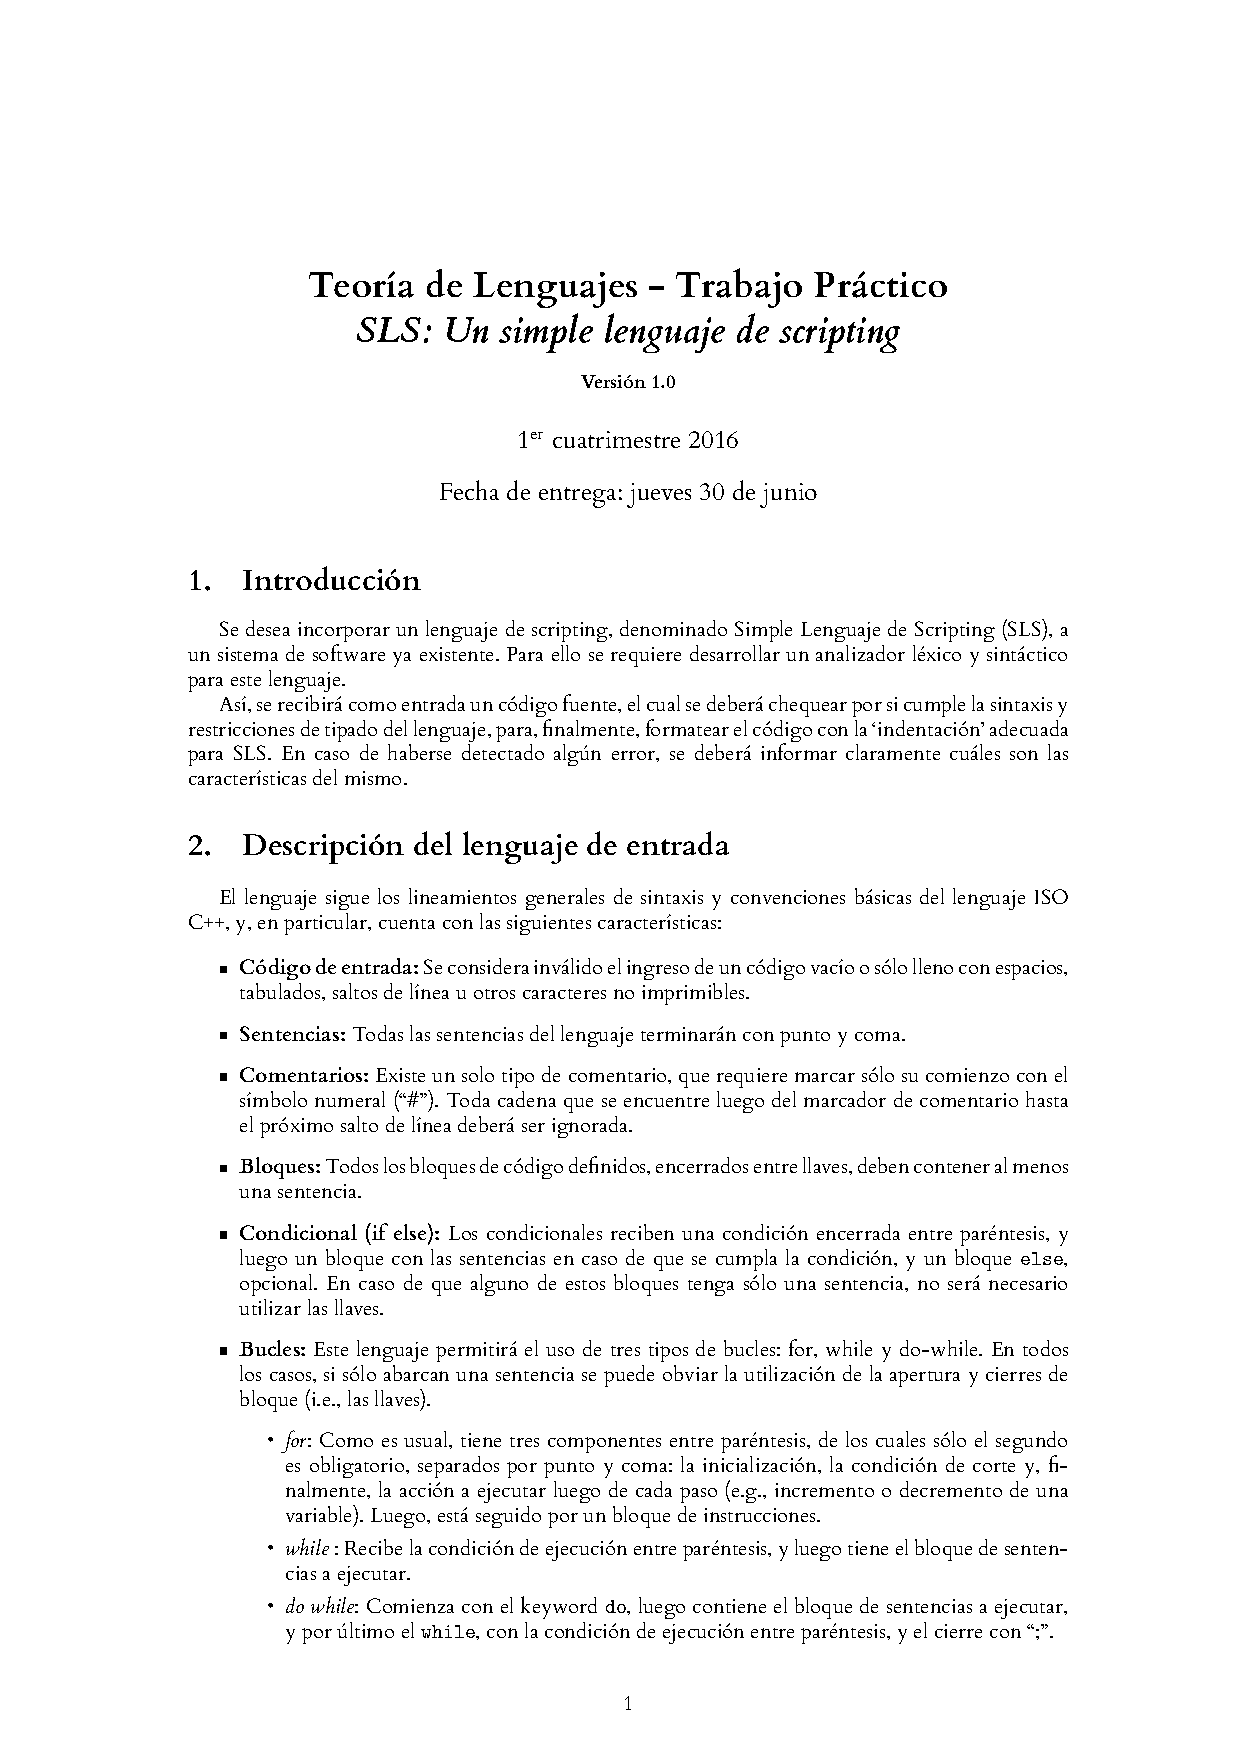
\includepdf[pages=-]{../enunciado/enunciado.pdf}
